%% ---------------------------------------------------------------------------
%% resultados.tex
%% Descripción del trabajo realizado (Resultados y análisis)
%% ---------------------------------------------------------------------------

\chapter{Descripción del trabajo realizado}
\label{ch:trabajo}



% ============================================================================
\section{Proceso para llegar a la solución aplicada}
\label{sec:trabajo_proceso}
% ============================================================================

Esta sección detalla el proceso metodológico de ingeniería seguido para diseñar e
implementar la solución, abordando secuencialmente cada uno de los objetivos
específicos definidos para el proyecto. Se describen las herramientas de
análisis empleadas, las abstracciones realizadas y las decisiones de diseño
fundamentales que permitieron construir la plataforma de evaluación.

% ---------------------------------------------------------------------------
\subsection{Implementación del módulo PLPUF en HDL}
\label{sec:proc_hdl}

El proceso de implementación del núcleo generador de entropía inició con la
abstracción del circuito PLPUF propuesto por Hori~et~al.~\cite{hori_2011_pseudolfsr}
hacia un modelo de descripción de hardware puramente combinacional. Se decidió
emplear el lenguaje Verilog, optando por una arquitectura parametrizable
que facilitara el ajuste del ancho del desafío (configurado a 128~bits) y las
posiciones de las compuertas lógicas de retroalimentación (polinomio primitivo).

Una decisión de diseño crítica en esta etapa fue cómo preservar el comportamiento
oscilatorio del circuito durante la síntesis. Las herramientas de síntesis (EDA),
como AMD Vivado, están diseñadas para optimizar la lógica combinacional y
eliminar bucles asíncronos que consideran como errores de diseño. Para evitar
que el sintetizador eliminara los inversores, que constituyen la fuente de
entropía física del sistema, se aplicaron restricciones de diseño explícitas.
Se utilizó el atributo \texttt{DONT\_TOUCH} sobre las celdas del núcleo para
prevenir la absorción de lógica, y la restricción \texttt{ALLOW\_COMBINATORIAL\_LOOPS}
en el archivo XDC para instruir a la herramienta que permitiera la existencia
del lazo cerrado. Estas decisiones
de síntesis fueron fundamentales para garantizar que el comportamiento analógico del
silicio (los retardos de propagación microscópicos de cada compuerta debidos a
las variaciones del proceso de fabricación) se preservara y pudiera ser
explotado en el entorno digital del FPGA.

% ---------------------------------------------------------------------------
\subsection{Desarrollo de la interfaz AXI-slave}
\label{sec:proc_axi}

Para habilitar el control del módulo PLPUF desde un procesador en un sistema
embebido, se aplicaron principios de diseño de interfaces estandarizadas,
seleccionando el protocolo AMBA AXI4-Lite por su ligereza y amplia adopción. El
diseño de la interfaz partió de la definición de un mapa de registros
\textit{memory-mapped I/O} (MMIO) estructurado. Se abstrajo el control del
hardware en 11~registros activos de 32~bits, organizados lógicamente para separar
funciones de configuración (desafío, duración de activación), control operativo
(inicio, reinicio) y estado (bancos de respuesta, banderas).

Una técnica de diseño clave aplicada durante el desarrollo de esta interfaz fue
la implementación de una lógica de prioridades de escritura en tres niveles.
Este enfoque garantizó que el hardware interno del PLPUF (prioridad alta) siempre
pudiera actualizar los registros de respuesta de forma segura y oportuna, evitando
condiciones de carrera o sobreescritura frente a las peticiones concurrentes del
procesador (prioridad baja/media). Esta abstracción aseguró que los registros
de respuesta se comportaran estrictamente como de «solo lectura» desde la
perspectiva del software. Finalmente, el código HDL integrado se sintetizó y se
empaquetó como un núcleo de propiedad intelectual (IP) reutilizable utilizando
Vivado IP Packager, estandarizando su instanciación para ser compatible con el
flujo de diseño gráfico de sistemas.

% ---------------------------------------------------------------------------
\subsection{Integración del sistema SoC}
\label{sec:proc_soc}

La síntesis del sistema completo se realizó empleando la herramienta Vivado IP
Integrator, aplicando el principio de diseño modular basado en componentes. Se
construyó el \textit{System-on-Chip} interconectando el módulo IP del PLPUF
(creado en la etapa anterior) con componentes de biblioteca estándar: el
procesador suave MicroBlaze~V (configurado con la arquitectura abierta RV32I para
eficiencia de área), bloques de memoria local BRAM de 64\,KB para
almacenamiento de instrucciones y datos, un controlador UART para comunicación
exterior, y el bloque AXI SmartConnect encargado del arbitraje y enrutamiento
de transacciones en el bus del sistema.

A nivel de \textit{software}, el proceso de integración involucró el desarrollo de
una arquitectura en capas utilizando la plataforma AMD Vitis. Se programó un
controlador (\textit{driver}) de bajo nivel en lenguaje C para abstraer las
direcciones físicas del hardware en una API de funciones intuitivas (como
\texttt{Plpuf\_SetChallenge} o \texttt{Plpuf\_Start}). Sobre esta capa de
abstracción, se construyeron las rutinas de \textit{firmware} para la validación
funcional y la evaluación exhaustiva. La decisión estratégica de trasladar la
lógica de recolección de datos masiva y los cálculos estadísticos preliminares, como el cómputo de respuestas de referencia (\textit{golden}) por votación
mayoritaria, directamente al microprocesador del SoC, permitió optimizar el
tiempo de ejecución del experimento y redujo sustancialmente el volumen de datos
transferidos hacia el computador anfitrión.

% ---------------------------------------------------------------------------
\subsection{Protocolo de evaluación estadística}
\label{sec:proc_eval}

El proceso de análisis para validar el desempeño de seguridad del módulo requirió
la definición y aplicación de un protocolo experimental riguroso, fundamentado en
el marco sistemático propuesto por Maiti~et~al.~\cite{maiti_2012_systematic}.
Se diseñó un experimento automatizado que ejecutó 10~ejecuciones independientes
sobre el sistema físico. Para estructurar adecuadamente el espacio de prueba,
se estableció para cada corrida un barrido sobre 10~duraciones de activación
diferentes ($c = 1, \ldots, 10$), evaluando en cada paso 20~desafíos
pseudoaleatorios fijos, a razón de 50~repeticiones por cada par
desafío-duración.

Este diseño metodológico garantizó la representatividad y significancia
estadística de los datos, acumulando aproximadamente 140\,000~evaluaciones del
PLPUF bajo condiciones operativas controladas. El cálculo final de las métricas
(uniformidad, confiabilidad, distancia de Hamming y efecto avalancha) se resolvió
mediante una estrategia híbrida: el preprocesamiento \textit{in-situ} en el FPGA
y el postprocesamiento en el computador anfitrión mediante \textit{scripts} de
Python, aprovechando librerías de visualización de datos para abstraer las
cifras tabulares en representaciones gráficas de análisis.


% ============================================================================
\section{Análisis de los resultados finales}
\label{sec:trabajo_resultados}
% ============================================================================

En esta sección se evidencia el análisis cuantitativo y cualitativo de los
resultados generados por el producto desarrollado. La presentación se divide en
correspondencia con la validación de cada objetivo específico, proporcionando
tablas y figuras que sustentan el grado de cumplimiento técnico y las
implicaciones de la plataforma.

% ---------------------------------------------------------------------------
\subsection{Implementación del módulo PLPUF en HDL}
\label{sec:res_oe1}

La validación del diseño HDL se centró en corroborar la viabilidad de
implementación en dispositivos con recursos limitados y en demostrar que el
circuito efectivamente genera respuestas no predecibles fundamentadas en la
entropía física del silicio.

La Tabla~\ref{tab:utilizacion_global} muestra la utilización de recursos extraída
del reporte de síntesis de Vivado tras la fase de \textit{place and route}.
El sistema SoC completo ocupa apenas el 12.29\,\% de las LUTs y el 6.37\,\% de los
\textit{flip-flops} disponibles en la FPGA Artix-7 \texttt{XC7A35T}, confirmando
que la solución es ampliamente implementable incluso en dispositivos modestos.

\begin{table}[htbp]
\centering
\caption{Utilización de recursos del sistema SoC completo sobre la FPGA
  Artix-7 \texttt{XC7A35T} tras la implementación física.}
\label{tab:utilizacion_global}
\small
\renewcommand{\arraystretch}{1.2}
\begin{tabular}{lrrr}
\hline
\textbf{Recurso} & \textbf{Usados} & \textbf{Disponibles} & \textbf{Util.\,(\%)} \\
\hline
\textit{Slice} LUTs                & 2\,556 & 20\,800 & 12.29 \\
\quad LUT como lógica              & 2\,449 & 20\,800 & 11.77 \\
\quad LUT como memoria             & 107    & 9\,600  & 1.11  \\
\textit{Slice} Registers           & 2\,650 & 41\,600 & 6.37  \\
\textit{Slices} ocupados           & 978    & 8\,150  & 12.00 \\
F7 Muxes                           & 83     & 16\,300 & 0.51  \\
F8 Muxes                           & 33     & 8\,150  & 0.40  \\
Bloques RAM (RAMB36E1)             & 16     & 50      & 32.00 \\
\hline
\end{tabular}
\end{table}

Para evaluar la eficiencia del módulo PLPUF de forma aislada, la
Tabla~\ref{tab:utilizacion_plpuf} reporta los recursos consumidos
exclusivamente por el periférico \texttt{axi\_plpuf\_0}. Requiere únicamente
484~LUTs (2.33\,\%) y 651~\textit{flip-flops} (1.56\,\%). De estos, 128~LUTs
corresponden a los inversores del núcleo combinacional preservados con el atributo
\texttt{DONT\_TOUCH}. Cabe destacar que el módulo no requiere bloques DSP ni
memoria BRAM, dejando estos recursos disponibles para funciones de aceleración
criptográfica en futuras aplicaciones.

\begin{table}[htbp]
\centering
\caption{Utilización de recursos del periférico AXI~PLPUF y del procesador
  MicroBlaze~V, según el reporte de síntesis individual.}
\label{tab:utilizacion_plpuf}
\small
\renewcommand{\arraystretch}{1.2}
\begin{tabular}{lrrrr}
\hline
\textbf{Componente} & \textbf{LUTs} & \textbf{FFs} & \textbf{F7/F8 Muxes} & \textbf{BRAM} \\
\hline
AXI PLPUF (\texttt{axi\_plpuf\_0})       & 484    & 651    & 64 / 32 & 0  \\
MicroBlaze~V (\texttt{microblaze\_riscv\_0}) & 1\,768 & 1\,285 & 19 / 1  & 0  \\
\hline
\end{tabular}
\end{table}

De forma más trascendente, el éxito del OE1 se demuestra mediante el
comportamiento estadístico de la uniformidad de bits en la salida (analizada
en detalle en la Sección~\ref{sec:res_oe4}). Dado que el circuito diseñado
es estricta y puramente lógico digital estándar, la única forma de que sus
salidas se asemejen a distribuciones pseudoaleatorias con proporciones de ceros y
unos balanceadas ($\sim$50\,\%) es debido a que la lógica está explotando con
éxito las minúsculas variaciones físicas de los retardos en los caminos de
los transistores. La ausencia de sesgo en las mediciones empíricas certifica
que las restricciones impuestas en Vivado funcionaron y el PLPUF extrae la
entropía inherente del hardware, en lugar de optimizarse hacia un estado constante.

% ---------------------------------------------------------------------------
\subsection{Pruebas de la interfaz AXI}
\label{sec:res_oe2}

Antes de realizar la evaluación masiva de seguridad, se realizaron pruebas de
validación funcional específicas (\texttt{test\_app1}) ejecutadas por el MicroBlaze~V
para comprobar rigurosamente el protocolo de comunicación de la interfaz AXI-slave.

En la Figura \ref{fig:results_test_app1} se reproduce la salida completa de la consola serie tras ejecutar la aplicación \texttt{test\_app1} en el hardware. Se observan claramente las cinco pruebas implementadas en el código:

\begin{enumerate}
  \item \textbf{Prueba de lectura/escritura de registros} (Test 1): Se escribe el valor 100 en el registro de duración y se lee posteriormente, obteniendo el mismo valor; análogamente, se escriben y leen sin alteración los registros de desafío (CHAL0 y CHAL1). Todos los pasos se muestran con el marcador \texttt{[PASS]}.
  
  \item \textbf{Evaluación única} (Test 2): Se lanza una operación PUF con un desafío fijo y se imprime la respuesta de 128 bits. La salida no es nula, lo que confirma que el núcleo genera una respuesta activa.
  
  \item \textbf{Prueba de repetibilidad} (Test 3): Se ejecuta cinco veces la misma operación (mismo desafío y misma duración, $c = 5$ por defecto). Las líneas etiquetadas como \texttt{Run:} muestran respuestas ligeramente diferentes en cada iteración.
  
  \item \textbf{Prueba de unicidad} (Test 4): Se comparan las respuestas para dos desafíos distintos. La salida muestra valores claramente diferentes (\texttt{Challenge A resp} vs. \texttt{Challenge B resp}), y el test declara \texttt{[PASS]} al no ser idénticas.
  
  \item \textbf{Barrido de duración} (Test 5): Se varía el parámetro de activación \(c\) de 1 a 10, y para cada valor se imprime la respuesta correspondiente. Se aprecia cómo cambia la salida al modificar la duración del pulso de activación.
\end{enumerate}

\begin{figure}[h]
  \centering
  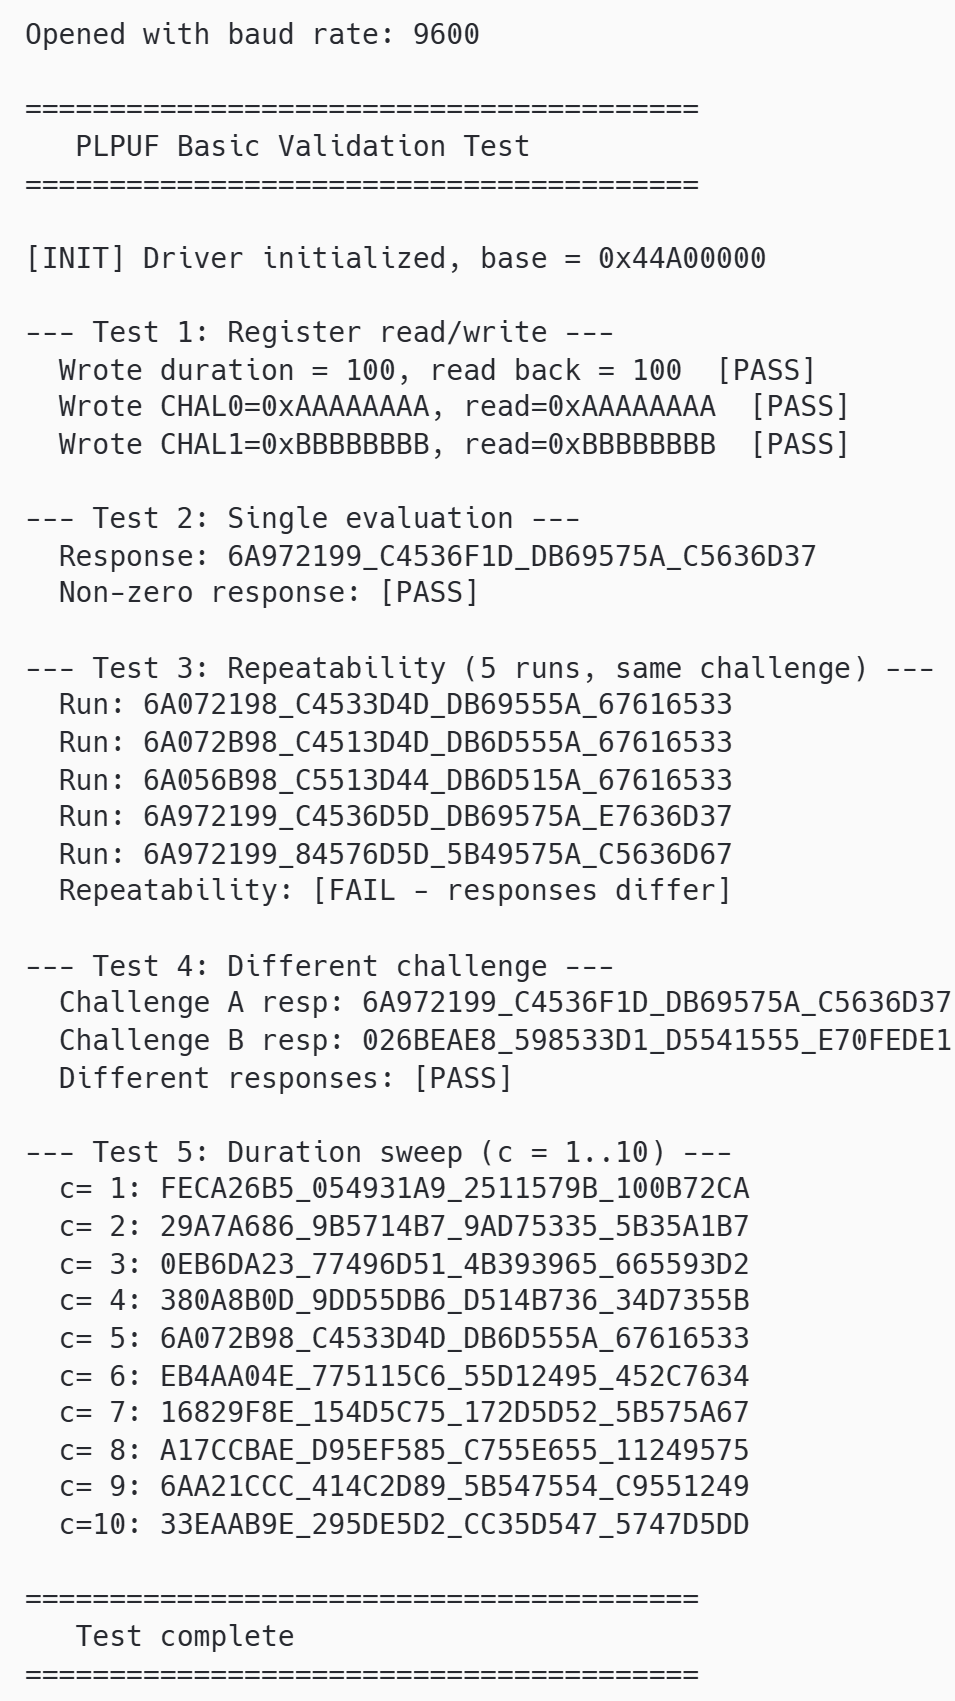
\includegraphics[width=0.48\textwidth]{Documento_TFG_EmanuelMarin/fig/results_test_app1.png}
  \caption{Resultados obtenidos al ejecutar \texttt{test\_app1}.}
  \label{fig:results_test_app1}
\end{figure}

% ---------------------------------------------------------------------------
\subsection{Prueba de integración del SoC}
\label{sec:res_oe3}

La prueba integral del SoC se comprobó mediante la ejecución exitosa de la
aplicación de evaluación exhaustiva (\texttt{test\_app2}). Esta prueba
demostró la correcta interoperabilidad de todos los componentes del sistema
trabajando en conjunto: el procesador MicroBlaze~V ejecutando el
\textit{firmware} desde la memoria BRAM, el bloque AXI SmartConnect
enrutando exitosamente las transacciones en el bus, el módulo PLPUF
respondiendo a las peticiones en hardware y el controlador UART
transmitiendo los resultados hacia el computador anfitrión.


La ejecución autónoma del protocolo permitió recolectar aproximadamente
140\,000~respuestas del sistema de forma ininterrumpida. La estabilidad
operacional lograda a lo largo de las 10~ejecuciones independientes evidencia
una comunicación bidireccional USB-UART con cero pérdida de información.
Esta prueba de resistencia (\textit{end-to-end}) constituye la evidencia
definitiva del logro exitoso del OE3 y confirma la conformación de un
sistema embebido estable, apto para el prototipado en seguridad de la
información.

Los resultados obtenidos para 1 de las 10 ejecuciones independientes de \texttt{test\_app2} se muestran en las Figuras~\ref{fig:results_test_app2_section_1} a~\ref{fig:results_test_app2_section_4}. En primer lugar, la Figura~\ref{fig:results_test_app2_section_1} recoge la verificación de la interfaz de registro y la funcionalidad de reinicio suave (\emph{soft reset}). Se observa que la lectura y escritura de los registros DURATION, CHAL\_0 y CHAL\_3 son correctas, mientras que el registro RESP\_0 se comporta como solo lectura (no permite escritura). Además, el reinicio suave limpia correctamente el bit \texttt{done} del registro de estado. Todos estos tests superan la validación, lo que confirma que el núcleo PLPUF responde adecuadamente a las transacciones del bus AXI y que la integración del sistema es sólida.

\begin{figure}[H]
  \centering
  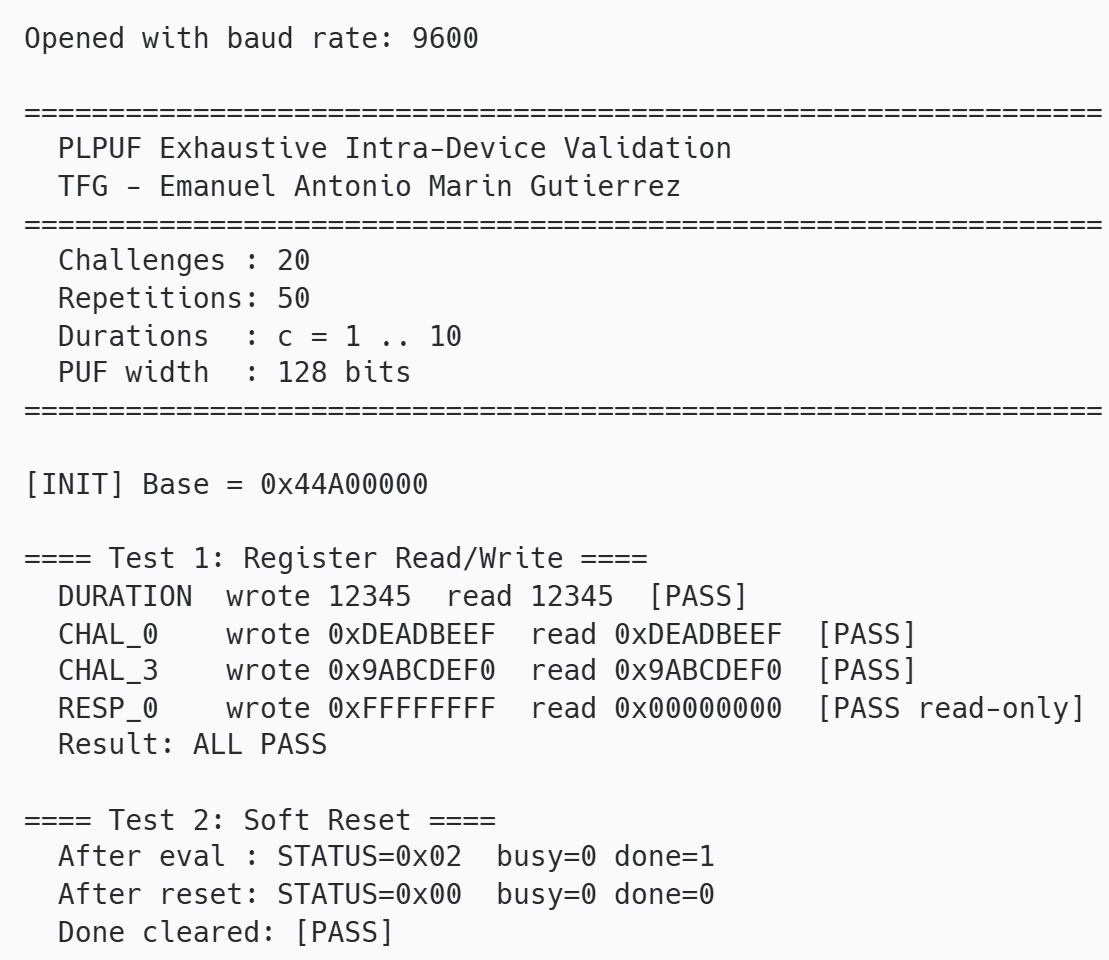
\includegraphics[width=0.65\textwidth]{Documento_TFG_EmanuelMarin/fig/results_test_app2_section_1.png}
  \caption{Verificación de la interfaz de registros y funcionalidad de reinicio suave.}
  \label{fig:results_test_app2_section_1}
\end{figure}

La Figura~\ref{fig:results_test_app2_section_2} presenta el barrido de duración de activación \(c\) desde 1 hasta 10. En ella se aprecia claramente la compensación entre fiabilidad y unicidad: para valores pequeños de \(c\) (1 a 4) la fiabilidad es superior al 95\,\% (BER inferior al 5\,\%), mientras que la uniformidad se mantiene muy próxima al 50\,\% ideal. A medida que aumenta \(c\), la fiabilidad desciende gradualmente hasta el 89\,\% para \(c=10\), y el IntraHD (distancia de Hamming intra-dispositivo) crece hasta 15.67, lo que indica una mayor inestabilidad de la respuesta. Por otra parte, el InterHD (distancia de Hamming entre diferentes desafíos) se aleja del 50\,\% ideal a medida que \(c\) aumenta, pasando de un 48.46\,\% en \(c=1\) a un 37.65\,\% en \(c=10\). Esto sugiere que para valores altos de \(c\) la respuesta del PUF se vuelve menos única y más dependiente del desafío.

\begin{figure}[H]
  \centering
  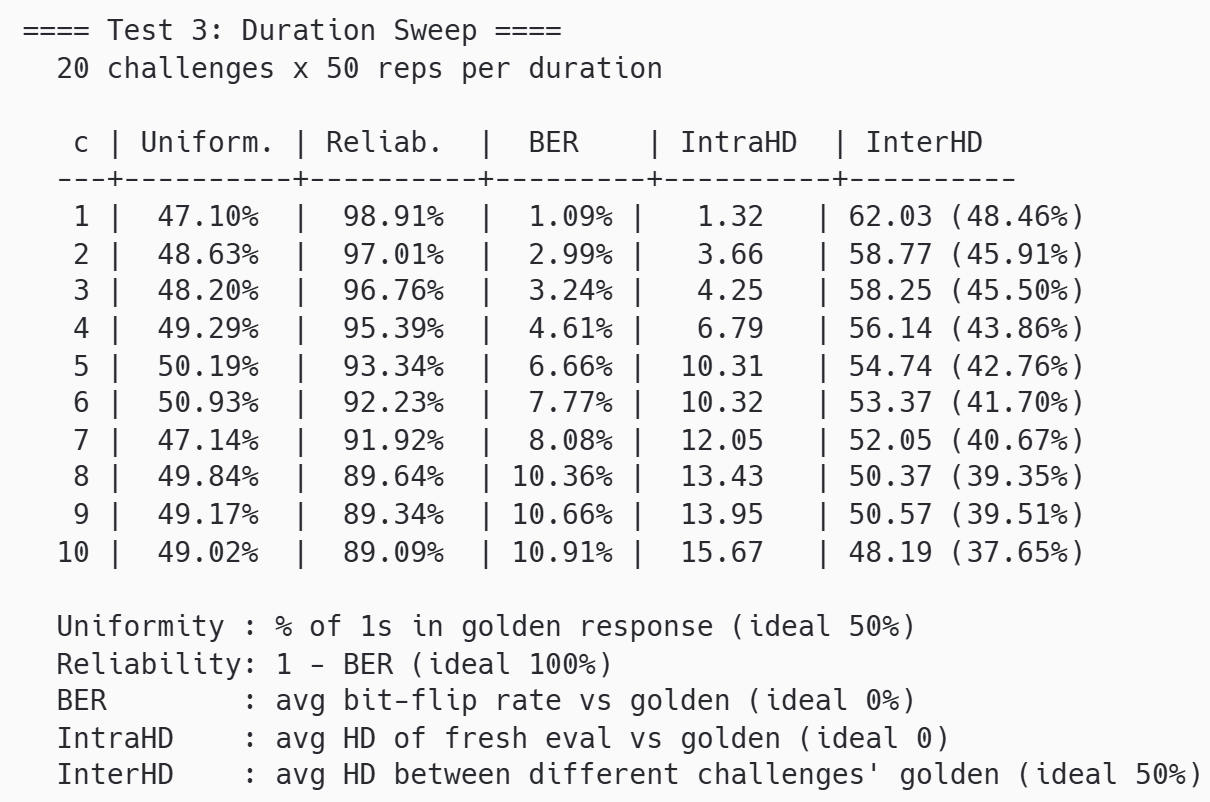
\includegraphics[width=0.9\textwidth]{Documento_TFG_EmanuelMarin/fig/results_test_app2_section_2.png}
  \caption{Barrido de duración de activación (\(c = 1 \ldots 10\)): uniformidad, fiabilidad, BER, IntraHD e InterHD.}
  \label{fig:results_test_app2_section_2}
\end{figure}

La Figura~\ref{fig:results_test_app2_section_3_1} muestra las 50 respuestas crudas obtenidas para el primer desafío con \(c=5\), junto con la respuesta \emph{golden} calculada por mayoría de votos. Se observan pequeñas variaciones entre las diferentes evaluaciones, como era de esperar por la presencia de ruido y metaestabilidad. Estas variaciones son consistentes con el BER de 6.66\,\% reportado en la Figura~\ref{fig:results_test_app2_section_2} para \(c=5\).

\begin{figure}[H]
  \centering
  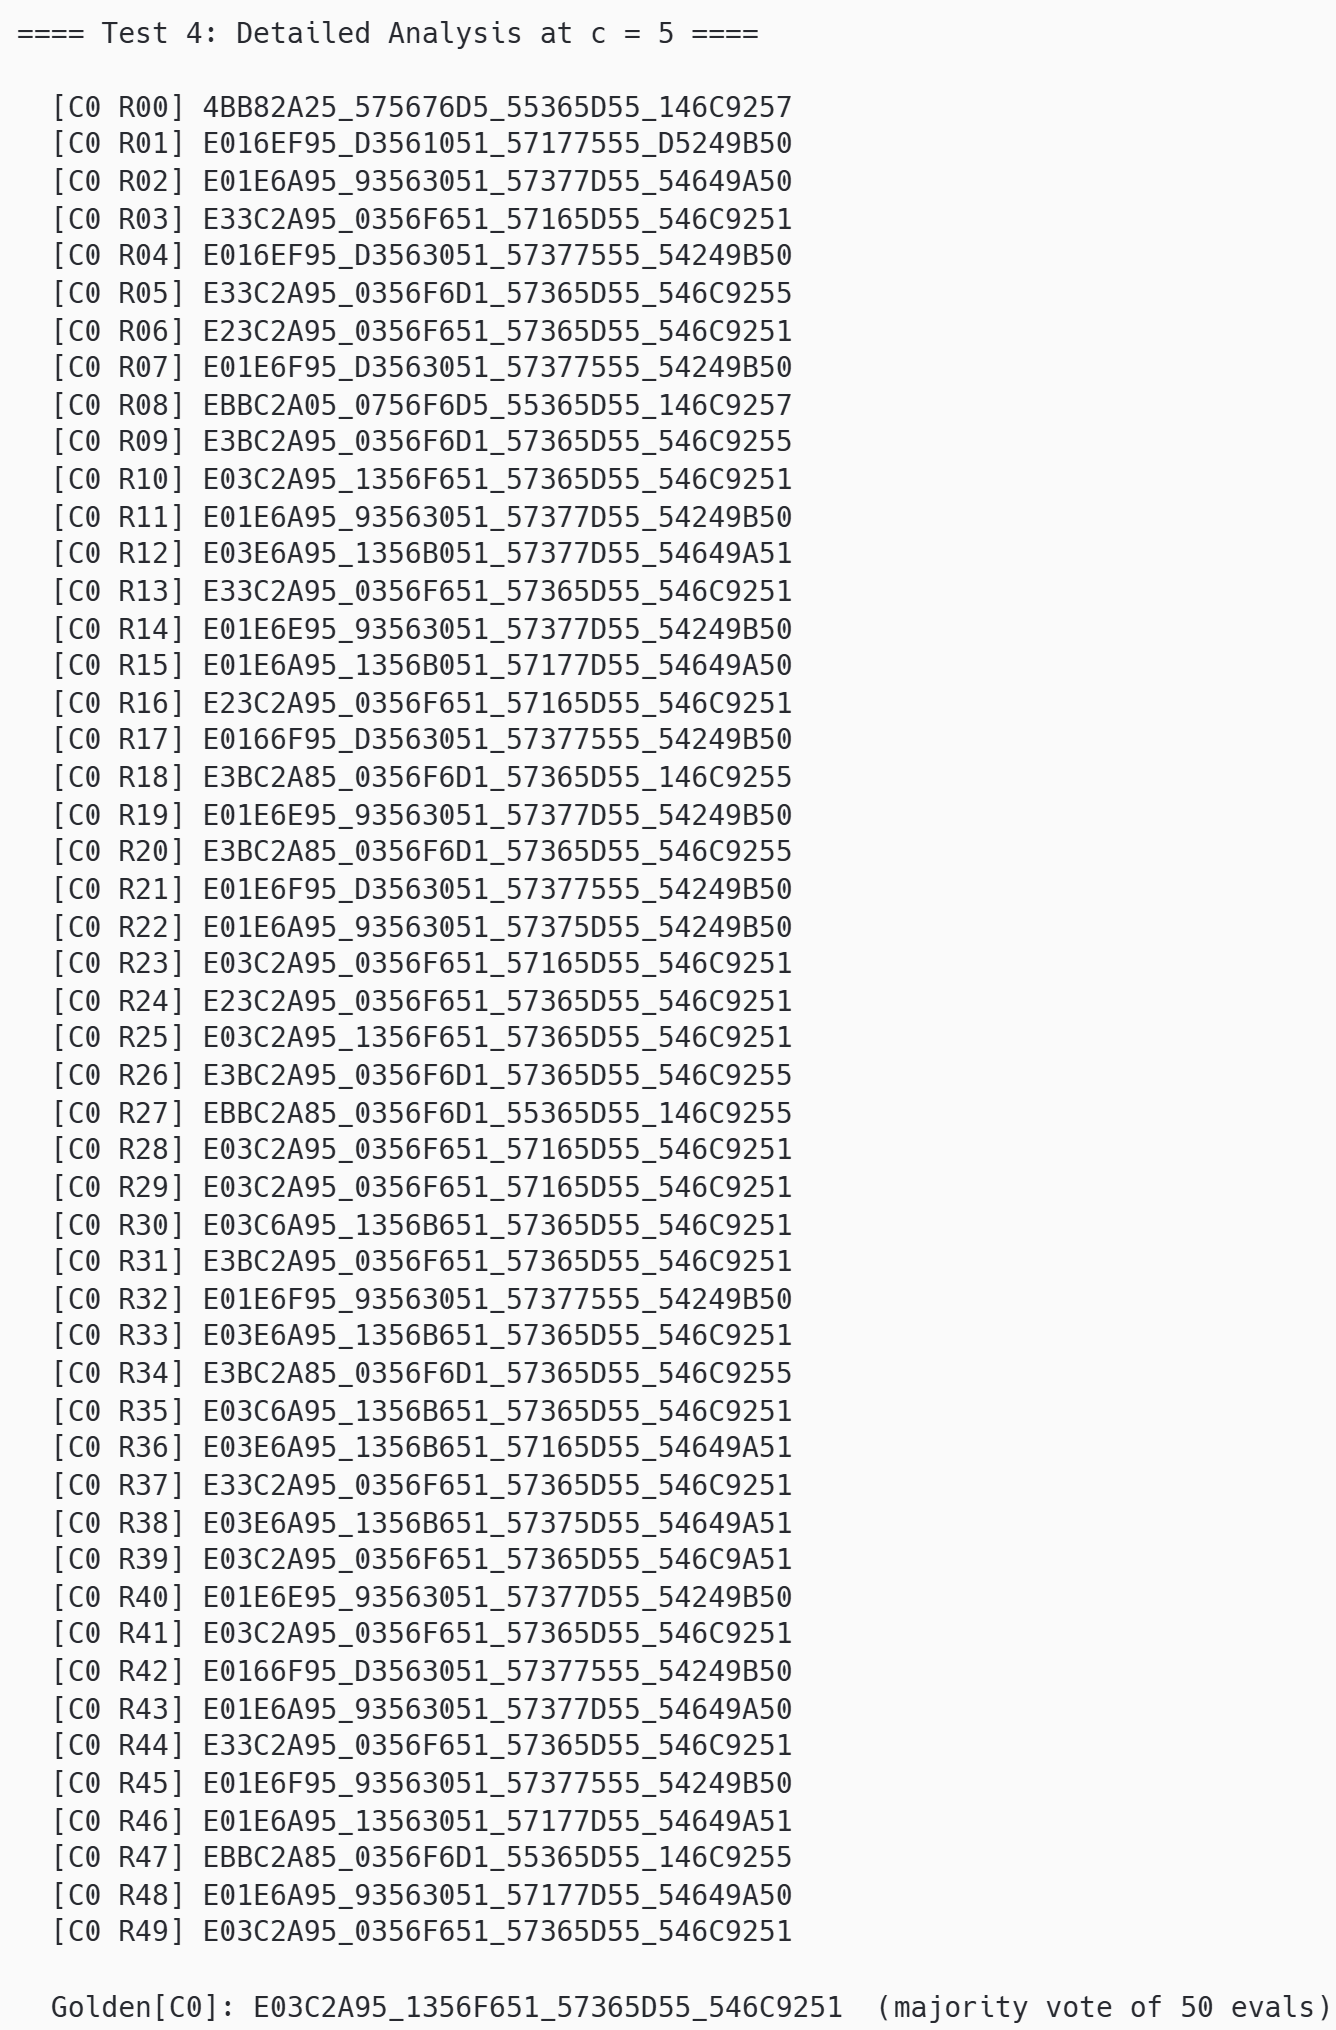
\includegraphics[width=0.7\textwidth]{Documento_TFG_EmanuelMarin/fig/results_test_app2_section_3_1.png}
  \caption{Respuestas crudas (50 evaluaciones) y respuesta \emph{golden} (mayoría de votos) para el desafío 0 con \(c = 5\).}
  \label{fig:results_test_app2_section_3_1}
\end{figure}

El análisis de estabilidad por bit y el histograma de distancias intra-dispositivo se presentan en la Figura~\ref{fig:results_test_app2_section_3_2}. En el mapa de estabilidad (parte superior) se asigna a cada bit un grado de fiabilidad del 0 (muy ruidoso) al 9 (muy estable). Se observa que 40 de los 128 bits son estables (fiabilidad \(\ge 95\,\%\)) y ningún bit es ruidoso (fiabilidad \(<80\,\%\)), lo que indica un comportamiento aceptable. El histograma de IntraHD (parte inferior) muestra que la mayoría de las distancias de Hamming entre una evaluación fresca y la respuesta \emph{golden} se concentran en los primeros 15 bits, con un máximo de 55 ocurrencias en el rango 5–9. No se registran distancias superiores a 29 bits, lo que confirma que las respuestas son bastante repetibles y que la mayoría de las variaciones son pequeñas.

\begin{figure}[H]
  \centering
  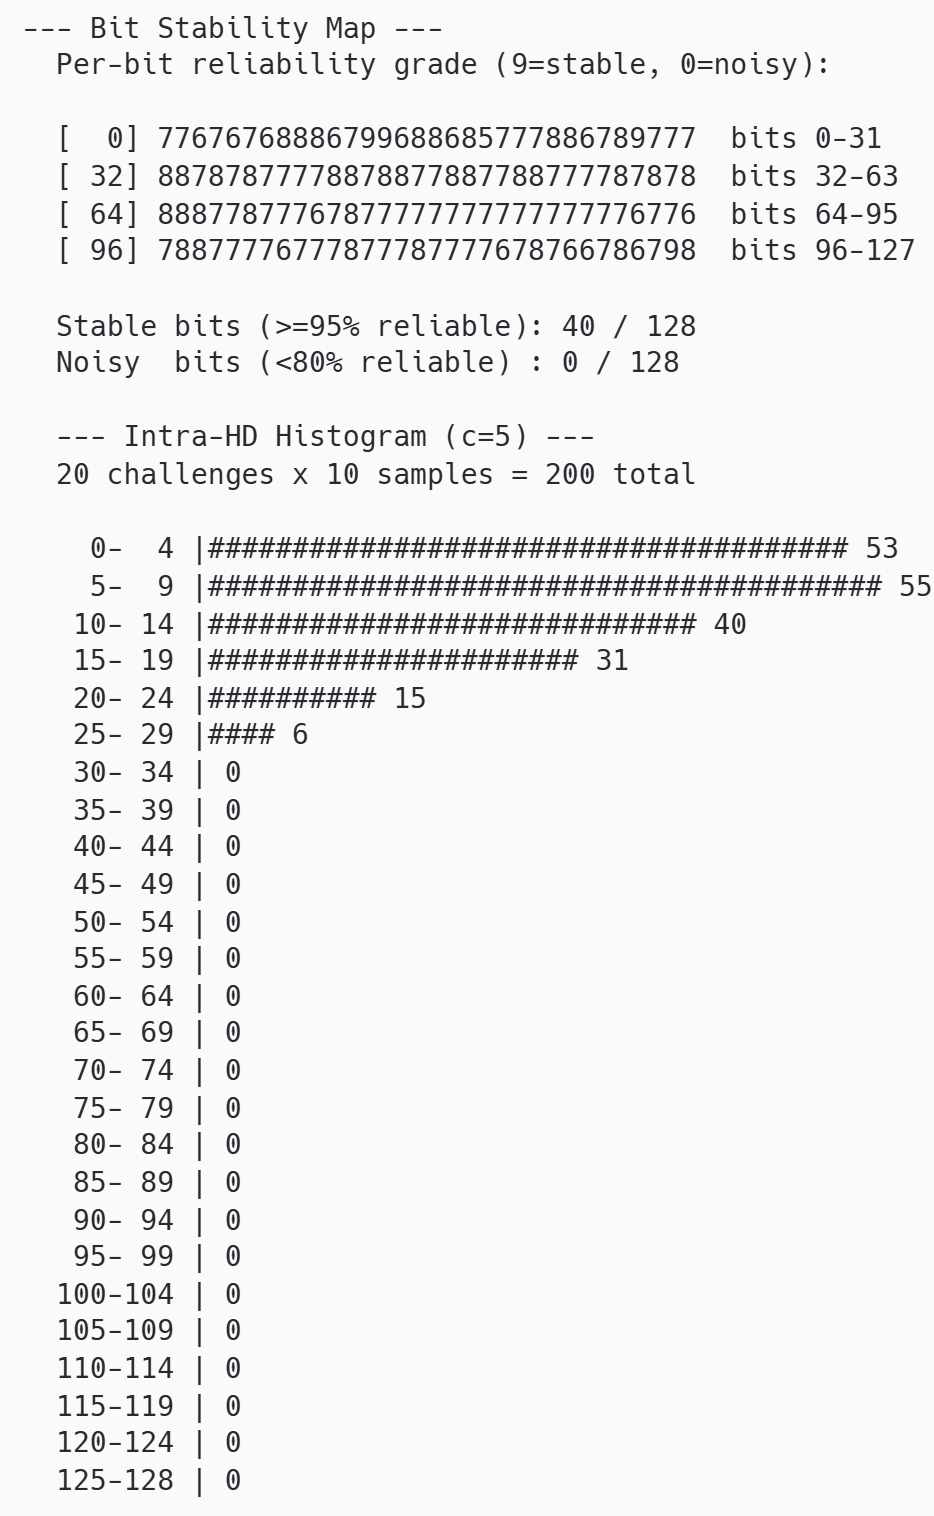
\includegraphics[width=0.68\textwidth]{Documento_TFG_EmanuelMarin/fig/results_test_app2_section_3_2.png}
  \caption{Mapa de estabilidad por bit (grado 9 = estable, 0 = ruidoso) e histograma de distancias de Hamming intra-dispositivo para \(c = 5\).}
  \label{fig:results_test_app2_section_3_2}
\end{figure}

Finalmente, la Figura~\ref{fig:results_test_app2_section_4} evalúa el efecto avalancha para \(c=5\). Se mide la distancia de Hamming entre la respuesta \emph{golden} del desafío base y la obtenida al modificar un único bit del desafío. El promedio de cambio observado es tan solo del 9.13\,\%, muy alejado del 50\,\% ideal que caracterizaría una función criptográficamente fuerte. Esto indica que el PLPUF implementado no presenta un efecto avalancha satisfactorio, lo cual es esperable por tratarse de un PUF basado en osciladores de anillo no lineal (no es una función hash). Este resultado deberá tenerse en cuenta si se pretende utilizar el PUF en aplicaciones que requieran una alta sensibilidad al cambio del desafío.

\begin{figure}[H]
  \centering
  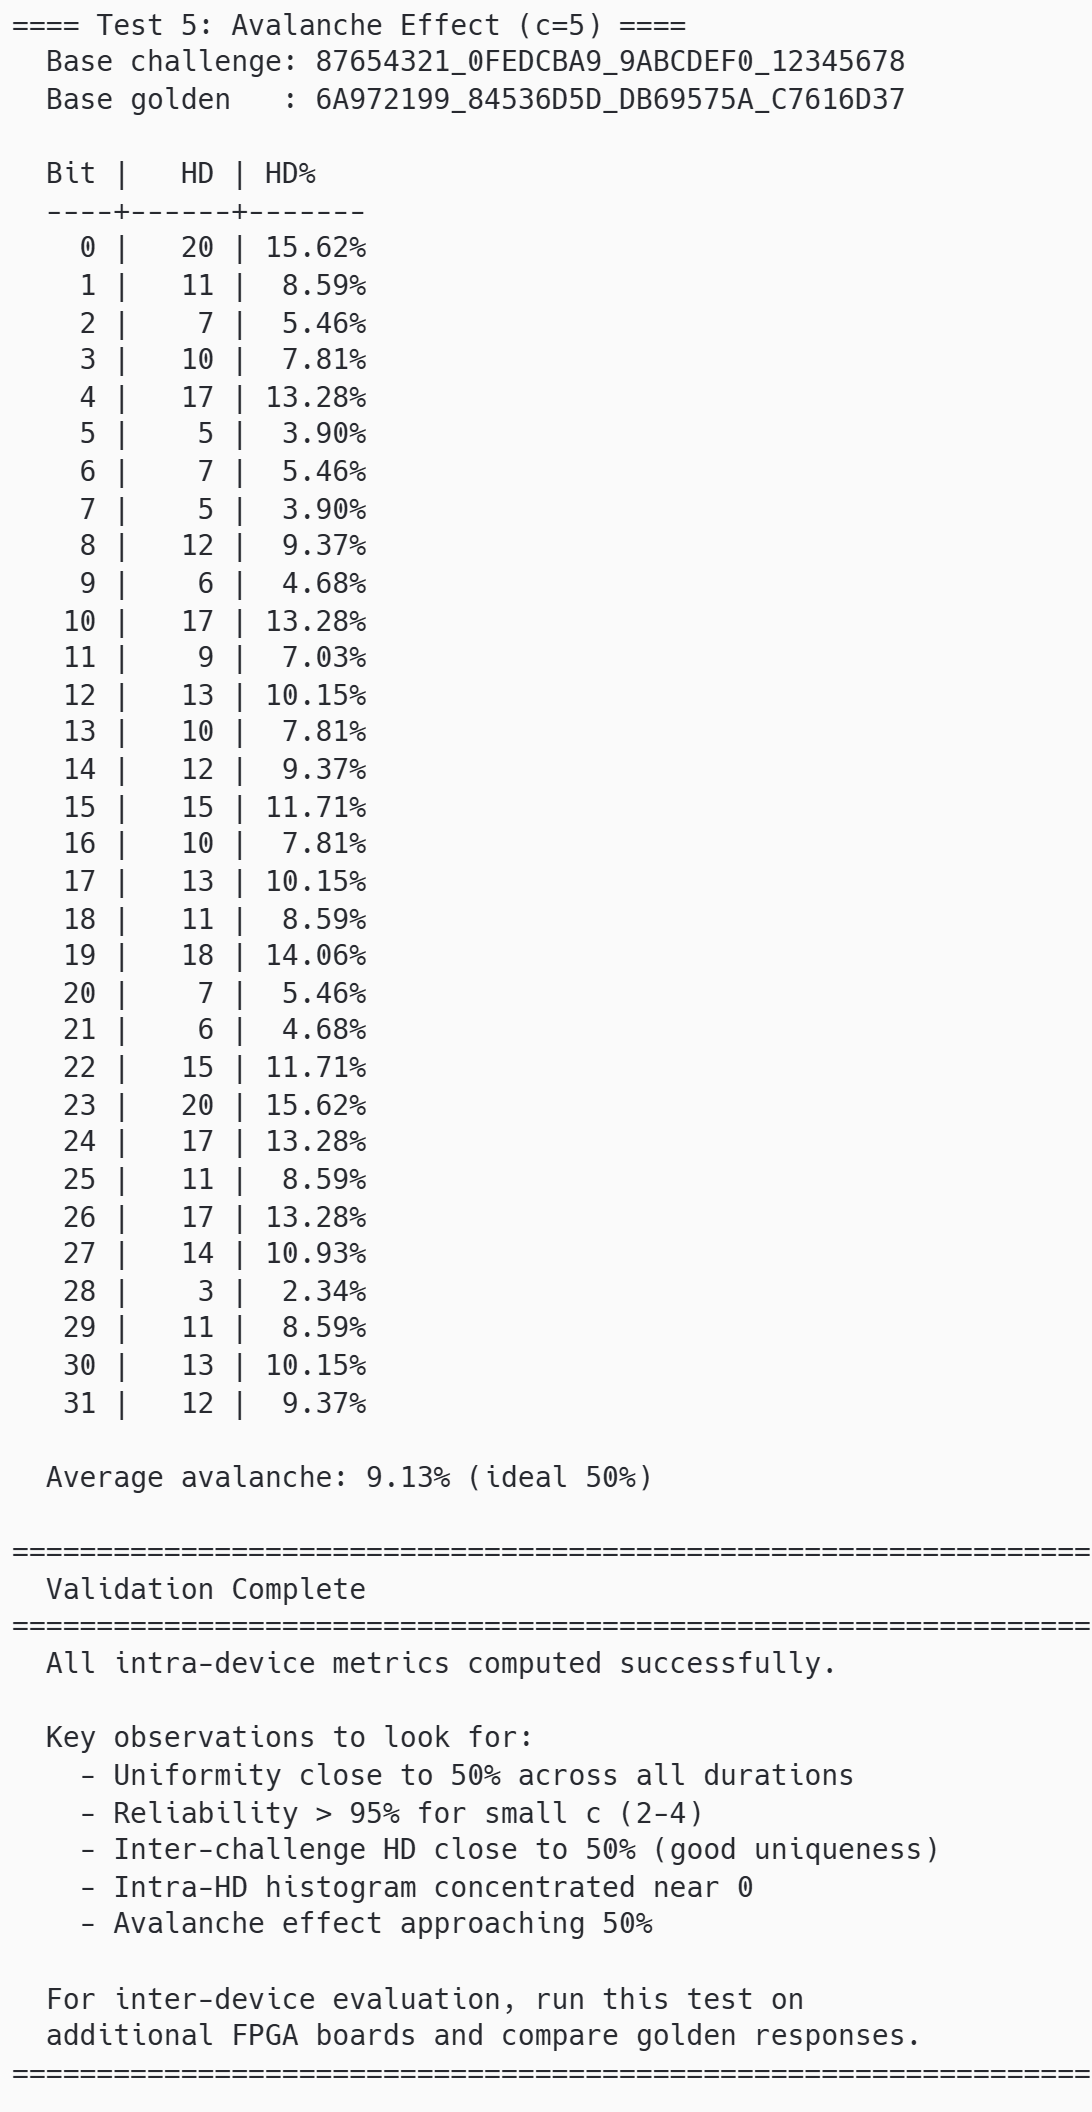
\includegraphics[width=0.7\textwidth]{Documento_TFG_EmanuelMarin/fig/results_test_app2_section_4.png}
  \caption{Efecto avalancha para \(c = 5\): distancia de Hamming (en bits y porcentaje) al modificar cada bit del desafío.}
  \label{fig:results_test_app2_section_4}
\end{figure}

% ---------------------------------------------------------------------------
\subsection{Resultados de la evaluación de seguridad}
\label{sec:res_oe4}

Es importante señalar que todas las pruebas corresponden a una evaluación
\textbf{intra-dispositivo}: se realizaron sobre un único chip FPGA
(Artix-7 \texttt{XC7A35T-1CPG236C}). La limitación de no contar con
placas adicionales fue declarada en la Sección~\ref{chp:intro}. La unicidad se
estima indirectamente mediante la distancia de Hamming inter-desafío.
Los valores reportados a continuación corresponden a la media $\pm$
desviación estándar calculadas sobre las 10~ejecuciones independientes.

\subsubsection{Resultados del barrido de duración}

La Tabla~\ref{tab:sweep_results} resume los resultados del barrido de
duración para las cinco métricas principales. La Figura~\ref{fig:res_summary}
presenta estos mismos datos de forma gráfica.

\begin{table}[htbp]
\centering
\caption{Resultados del barrido de duración (media $\pm$ desviación estándar,
  $n=10$ ejecuciones, 20~desafíos $\times$ 50~repeticiones por corrida).}
\label{tab:sweep_results}
\small
\renewcommand{\arraystretch}{1.2}
\begin{tabular}{c r@{$\,\pm\,$}l r@{$\,\pm\,$}l r@{$\,\pm\,$}l
                  r@{$\,\pm\,$}l r@{$\,\pm\,$}l}
\hline
$c$ &
\multicolumn{2}{c}{Unif.\,(\%)} &
\multicolumn{2}{c}{Conf.\,(\%)} &
\multicolumn{2}{c}{BER\,(\%)} &
\multicolumn{2}{c}{Intra-HD (bits)} &
\multicolumn{2}{c}{Inter-HD\,(\%)} \\
\hline
 1 & 47.10 & 0.04 & 98.97 & 0.03 &  1.03 & 0.03 &  1.31 & 0.06 & 48.48 & 0.06 \\
 2 & 48.68 & 0.09 & 97.09 & 0.07 &  2.91 & 0.07 &  3.92 & 0.30 & 46.03 & 0.07 \\
 3 & 47.93 & 0.19 & 96.81 & 0.06 &  3.19 & 0.06 &  4.63 & 0.24 & 45.63 & 0.10 \\
 4 & 49.27 & 0.13 & 95.13 & 0.15 &  4.87 & 0.15 &  6.73 & 0.34 & 44.04 & 0.16 \\
 5 & 50.14 & 0.14 & 93.38 & 0.13 &  6.62 & 0.13 &  9.40 & 0.52 & 42.55 & 0.14 \\
 6 & 51.07 & 0.19 & 92.66 & 0.23 &  7.34 & 0.23 & 10.72 & 0.72 & 41.93 & 0.16 \\
 7 & 47.30 & 0.19 & 91.99 & 0.12 &  8.01 & 0.12 & 11.72 & 0.47 & 40.81 & 0.17 \\
 8 & 49.95 & 0.23 & 89.89 & 0.30 & 10.11 & 0.30 & 13.39 & 0.54 & 39.53 & 0.18 \\
 9 & 49.20 & 0.22 & 89.64 & 0.34 & 10.36 & 0.34 & 14.35 & 0.41 & 39.39 & 0.23 \\
10 & 49.24 & 0.17 & 88.65 & 0.23 & 11.36 & 0.23 & 15.62 & 0.54 & 37.93 & 0.29 \\
\hline
\end{tabular}
\end{table}

\begin{figure}[htbp]
  \centering
  
\includegraphics[width=\textwidth]{fig/res_summary_4panel.pdf}
  \caption{Resumen de métricas del PLPUF en función de la duración de
    activación~$c$. Las barras de error representan $\pm 1\sigma$ sobre
    10~ejecuciones independientes. (a)~Uniformidad, (b)~Confiabilidad,
    (c)~HD intra-dispositivo, (d)~HD inter-desafío.}
  \label{fig:res_summary}
\end{figure}

\subsubsection{Uniformidad}

La uniformidad mide la proporción de unos en la respuesta \textit{golden}
del PLPUF; el valor ideal es 50\,\%, lo que indica máxima entropía por
bit~\cite{maiti_2012_systematic}. Como se muestra en la
Figura~\ref{fig:res_uniformity}, la uniformidad promedio se mantiene entre
47.10\,\% ($c = 1$) y 51.07\,\% ($c = 6$) a lo largo de todas las duraciones
de activación, con una desviación estándar inferior a 0.25 puntos porcentuales.
Este comportamiento confirma la ausencia de sesgos sistemáticos en el hardware,
comprobando el requerimiento analizado en la Sección~\ref{sec:res_oe1}.

\begin{figure}[htbp]
  \centering
  
\includegraphics[width=0.76\textwidth]{fig/res_uniformity.pdf}
  \caption{Uniformidad del PLPUF en función de la duración de activación~$c$
    (media $\pm 1\sigma$, $n=10$). La línea discontinua roja indica el valor
    ideal de 50\,\%.}
  \label{fig:res_uniformity}
\end{figure}

\subsubsection{Confiabilidad y tasa de error de bit (BER)}

La confiabilidad cuantifica la reproducibilidad de las respuestas ante el
mismo desafío~\cite{maiti_2012_systematic}. La Figura~\ref{fig:res_reliability_ber}
muestra la evolución de ambas métricas en función de la duración de activación.
Se observa una relación inversa: para $c = 1$, la confiabilidad alcanza
$98.97 \pm 0.03$\,\%, mientras que para $c = 10$ desciende a
$88.65 \pm 0.23$\,\%. Para $c \leq 4$, la confiabilidad se mantiene por encima del
95\,\%, umbral considerado aceptable para identificación de
dispositivos~\cite{hori_2011_pseudolfsr}. La configuración $c = 1$ resulta ser la
más confiable con un BER de $1.03 \pm 0.03$\,\%.

La degradación con el aumento de~$c$ se explica por la naturaleza del lazo
combinacional: la oscilación prolongada causa una acumulación exponencial de ruido
térmico en el circuito lógico, perturbando la evaluación final y generando una
menor fiabilidad intrínseca~\cite{hori_2011_pseudolfsr}.

\begin{figure}[htbp]
  \centering
  
\includegraphics[width=0.85\textwidth]{fig/res_reliability_ber.pdf}
  \caption{Confiabilidad (eje izquierdo) y BER (eje derecho) en función de la
    duración de activación~$c$ (media $\pm 1\sigma$, $n=10$).}
  \label{fig:res_reliability_ber}
\end{figure}

\subsubsection{Distancia de Hamming intra-dispositivo e inter-desafío}

La distancia de Hamming (HD) intra-dispositivo ideal es 0~bits, representando
reproducibilidad perfecta. Para $c = 1$, la HD intra-dispositivo es de
$1.31 \pm 0.06$~bits (1.02\,\% de la respuesta), consistente con la literatura.
A medida que~$c$ aumenta, crece hasta $15.62 \pm 0.54$~bits ($\sim$12.2\,\%)
para $c = 10$ (Figura~\ref{fig:res_intra_hd}).

\begin{figure}[htbp]
  \centering
  
\includegraphics[width=0.85\textwidth]{fig/res_intra_hd.pdf}
  \caption{Distancia de Hamming intra-dispositivo promedio en función de la
    duración de activación~$c$ (media $\pm 1\sigma$, $n=10$).}
  \label{fig:res_intra_hd}
\end{figure}

La distancia de Hamming inter-desafío (ideal 50\,\%) se empleó como alternativa
evaluativa a la carencia de métricas multi-chip. Como muestra la
Figura~\ref{fig:res_inter_hd}, en $c = 1$ fue de $48.48 \pm 0.06$\,\%. Con el
aumento de~$c$ disminuye a $37.93 \pm 0.29$\,\% en $c = 10$. Esto implica que a
mayores duraciones, los patrones lógicos tienden a colisionar y reducir la
diversidad criptográfica en la firma de salida del PLPUF.

\begin{figure}[htbp]
  \centering
  
\includegraphics[width=0.78\textwidth]{fig/res_inter_hd.pdf}
  \caption{Distancia de Hamming inter-desafío (como porcentaje de los
    128~bits) en función de la duración de activación~$c$ (media $\pm
    1\sigma$, $n=10$). La línea discontinua roja indica el ideal de 50\,\%.}
  \label{fig:res_inter_hd}
\end{figure}

\subsubsection{Análisis detallado a $c = 5$ y efecto avalancha}

La duración $c = 5$ se seleccionó como punto representativo de análisis medio.
Un análisis del mapa de estabilidad sobre las 10~ejecuciones indicó un promedio
de $39.5 \pm 3.8$ bits altamente estables y apenas $0.5 \pm 0.5$ bits
sistemáticamente ruidosos, requiriendo algoritmos correctores (Helper Data)
para estabilización determinista en aplicaciones prácticas. El histograma
de distancia no excedió los 29~bits de error bajo ninguna evaluación de prueba.

Respecto al efecto avalancha (Figura~\ref{fig:res_avalanche}), el porcentaje
promedio observado de cambio en los bits de respuesta al alternar un solo bit del
desafío de entrada fue del $8.43 \pm 1.15$\,\%, inferior al 50\,\% requerido por
la criptografía moderna. Este bajo grado de difusión es atribuible a las limitantes
arquitectónicas del polinomio matemático de estructura Fibonacci implementado
\cite{alsharkawy_2024_plpufs}.

\begin{figure}[htbp]
  \centering
  
\includegraphics[width=0.80\textwidth]{fig/res_avalanche.pdf}
  \caption{Efecto avalancha del PLPUF a $c = 5$: porcentaje de bits que
    cambian en la respuesta al invertir un solo bit del desafío (media $\pm
    1\sigma$, $n=10$). La línea discontinua roja indica el ideal de 50\,\% y
    la línea punteada verde el promedio observado.}
  \label{fig:res_avalanche}
\end{figure}

% ---------------------------------------------------------------------------
\subsection{Comparación con referencias y discusión general}
\label{sec:res_discusion}

La Tabla~\ref{tab:comparacion} enmarca los resultados de la plataforma actual
frente a los hallazgos iniciales documentados por Hori~et~al.~\cite{hori_2011_pseudolfsr}.

\begin{table}[htbp]
\centering
\caption{Comparación de resultados con la evaluación de referencia de
  Hori~et~al.~\cite{hori_2011_pseudolfsr}.}
\label{tab:comparacion}
\small
\renewcommand{\arraystretch}{1.3}
\begin{tabular}{lcc}
\hline
\textbf{Parámetro} &
\textbf{Este trabajo} &
\textbf{Hori et al.~\cite{hori_2011_pseudolfsr}} \\
\hline
Plataforma FPGA       & Artix-7 (\texttt{XC7A35T}) & Virtex-5 (\texttt{XC5VLX30}) \\
Frecuencia de reloj   & 100\,MHz           & 24\,MHz \\
Ancho del PLPUF       & 128~bits           & 128~bits \\
Dispositivos evaluados & 1                 & 16 \\
Desafíos por dispositivo & 20              & 100 \\
Repeticiones por CRP  & 50                 & 100 \\
HD intra ($c=1$)      & 1.31~bits          & 1.76~bits \\
Confiabilidad ($c=1$) & 98.97\,\%          & $\sim$98.6\,\% \\
HD inter-desafío ($c=1$) & 48.48\,\%       & --- \\
HD inter-dispositivo  & No evaluada        & $\sim$50\,\% \\
\hline
\end{tabular}
\end{table}

Los hallazgos demuestran una alta concordancia con las capacidades teóricas del
diseño. La distancia de error promedio (1.31 bits) es inclusive menor que los 1.76
bits en \cite{hori_2011_pseudolfsr}, infiriendo que la familia Artix-7 a 100~MHz
produce una mayor resiliencia ante el entorno. La repetibilidad es alta
y confirma empíricamente la viabilidad de utilización para arquitecturas ligeras de
Hardware de Confianza (Hardware Root of Trust).

Los resultados de este capítulo constatan de manera ineludible que la duración
de la activación (el parámetro `$c$') actúa como el modulador de control entre
seguridad de entropía y consistencia operacional. Las operaciones en torno a
$c=1$ resultan óptimas para tareas criptográficas, mientras que valores ascendentes
erosionan el espacio de distinción de la firma resultante.

La principal limitación identificada fue la falta de evaluación
inter-dispositivo en un grupo poblacional, lo cual impidió una cuantificación
rigurosa del alias de bit como señalan las directrices de Maiti y Wilde
\cite{maiti_2012_systematic, wilde_2020_confidence}. Sin embargo, este
ejercicio demostró que a nivel constructivo, desde su descripción y control
por un SoC empotrado, un módulo PLPUF abierto resulta factible y ofrece las
propiedades mínimas de aleatoriedad local necesarias.

%%% Local Variables:
%%% mode: latex
%%% TeX-master: "main"
%%% End:
